% !TeX program = xelatex
\documentclass[a4paper,10pt]{article}

% ============================================================================
% ១. កញ្ចប់បណ្ណាល័យ និងការកំណត់ទំព័រ (Packages & Page Setup — តាមគំរូ ls_plan.tex)
% ============================================================================
\usepackage[a4paper, left=0.95cm, right=0.95cm, top=0.85cm, bottom=0.92cm, footskip=0.52cm]{geometry}
\usepackage{amsmath}
\usepackage{unicode-math}
\usepackage{fontspec}
\usepackage{longtable, array, multirow, colortbl}
\usepackage[table]{xcolor}
\usepackage{enumitem}
\usepackage{pifont}
\usepackage{fancyhdr}
\usepackage{tikz}
\usetikzlibrary{calc, arrows.meta, decorations.pathreplacing, patterns, positioning, babel}

\makeatletter
\let\@expl@@@mark@update@singlecol@structures@@\relax
\makeatother

% --- ប្រព័ន្ធស្វែងរកទីតាំងពុម្ពអក្សរស្វ័យប្រវត្តិ (Windows Local + Cloud Repo fonts/) ---
\providecommand{\NGSFindFonts}{%
  \IfFileExists{C:/Windows/Fonts/cambria.ttc}{%
    \def\NGSSysPath{C:/Windows/Fonts/}%
    \def\NGSUserPath{C:/Users/KIT/AppData/Local/Microsoft/Windows/Fonts/}%
  }{%
    \IfFileExists{./fonts/KhmerOSsiemreap.ttf}{\def\NGSSysPath{./fonts/}\def\NGSUserPath{./fonts/}}{%
    \IfFileExists{../fonts/KhmerOSsiemreap.ttf}{\def\NGSSysPath{../fonts/}\def\NGSUserPath{../fonts/}}{%
    \IfFileExists{../../fonts/KhmerOSsiemreap.ttf}{\def\NGSSysPath{../../fonts/}\def\NGSUserPath{../../fonts/}}{%
    \IfFileExists{../../../fonts/KhmerOSsiemreap.ttf}{\def\NGSSysPath{../../../fonts/}\def\NGSUserPath{../../../fonts/}}{%
    \IfFileExists{../../../../fonts/KhmerOSsiemreap.ttf}{\def\NGSSysPath{../../../../fonts/}\def\NGSUserPath{../../../../fonts/}}{%
    \IfFileExists{../../../../../fonts/KhmerOSsiemreap.ttf}{\def\NGSSysPath{../../../../../fonts/}\def\NGSUserPath{../../../../../fonts/}}{%
    \IfFileExists{../../../../../../fonts/KhmerOSsiemreap.ttf}{\def\NGSSysPath{../../../../../../fonts/}\def\NGSUserPath{../../../../../../fonts/}}{%
      \def\NGSSysPath{../../../../../../../fonts/}\def\NGSUserPath{../../../../../../../fonts/}%
    }}}}}}}%
  }%
}
\NGSFindFonts

% ============================================================================
% ២. កំណត់ពុម្ពអក្សរ (Fonts — តាមគំរូ ls_plan.tex)
% ============================================================================
\setmathfont[Path={\NGSSysPath}, FontIndex=1, Scale=1.02]{cambria.ttc}
\defaultfontfeatures{Ligatures=TeX}

\setmainfont[
  Path={\NGSUserPath},
  Extension=.ttf,
  Script=Khmer,
  BoldFont={KhmerOSsiemreap},
  BoldFeatures={FakeBold=1.8},
  ItalicFont={KhmerOSsiemreap},
  ItalicFeatures={FakeSlant=0.25},
  BoldItalicFont={KhmerOSsiemreap},
  BoldItalicFeatures={FakeBold=1.8, FakeSlant=0.25}
]{KhmerOSsiemreap}

\newfontfamily\muol[Path={\NGSUserPath}, Extension=.ttf, Script=Khmer]{KhmerOSmuollight}
\newfontfamily\Tacteing[Path={\NGSUserPath}, Extension=.TTF]{TACTENG}
\newfontfamily\TimesEn[Path={\NGSSysPath}, Extension=.ttf, BoldFont={timesbd}, ItalicFont={timesi}, BoldItalicFont={timesbi}]{times}
\newfontfamily\CalibriFont[Path={\NGSSysPath}, Extension=.ttf]{calibri}
\newfontfamily\CourierCirc[Path={\NGSSysPath}, Extension=.ttf]{cour}

\XeTeXlinebreaklocale "km"
\XeTeXlinebreakskip = 0pt plus 1pt minus 0.1pt

% ============================================================================
% ៣. ពណ៌ និងការតុបតែង (Colors & Styles)
% ============================================================================
\definecolor{stepbg}{HTML}{D9D9D9}
\definecolor{headgray}{HTML}{E6E6E6}
\definecolor{emphred}{HTML}{C00000}

\pagestyle{fancy}
\fancyhf{}
\renewcommand{\headrulewidth}{0pt}
\fancyfoot[R]{\CalibriFont\fontsize{9pt}{11pt}\selectfont\thepage}

\setlength{\parindent}{0pt}
\setlength{\parskip}{0pt}
\setlength{\tabcolsep}{4.5pt}
\setlength{\LTpre}{2pt}
\setlength{\LTpost}{2pt}

\newcolumntype{L}[1]{>{\raggedright\arraybackslash}p{#1}}
\newcolumntype{C}[1]{>{\centering\arraybackslash}p{#1}}

% ============================================================================
% ៤. ពាក្យបញ្ជាជំនួយ (Helper Macros)
% ============================================================================
\newcommand{\en}[1]{{\TimesEn #1}}
\newcommand{\enbf}[1]{{\TimesEn\bfseries #1}}
\newcommand{\khmflourish}{{\Tacteing\fontsize{15pt}{15pt}\selectfont 3}}
\newcommand{\wcirc}{{\CourierCirc\fontsize{9.5pt}{11pt}\selectfont o}}
\newcommand{\ditem}{{\fontsize{7.5pt}{10pt}\selectfont\ding{117}}\ }
\newcommand{\fiveE}[1]{\textcolor{emphred}{\CalibriFont\bfseries #1}}
\newcommand{\redsub}[1]{\textcolor{emphred}{#1}}
\newcommand{\timenote}[1]{\textcolor{emphred}{\textit{#1}}}
\newcommand{\stepheader}[1]{\multicolumn{3}{|c|}{\cellcolor{stepbg}\muol #1} \\ \hline}
\newcommand{\cfig}[1]{{\centering\vspace{3pt}#1\vspace{3pt}\par}}
\newcommand{\cnum}[1]{\mbox{\fontsize{10.5pt}{12pt}\selectfont\ding{\numexpr181+#1\relax}}}
\newcommand{\unit}[1]{\,\text{\en{#1}}}
\newcommand{\riel}{\,\text{៛}}
\newcommand{\graybox}[1]{\colorbox{headgray}{\strut #1}}

% ============================================================================
% ៥. រូបភាព TikZ ស-ខ្មៅ សម្រាប់បង្រៀនលើក្ដារខៀន និងសន្លឹកកិច្ចការ (B&W Diagrams)
% ============================================================================

% ១. E1 Engage: បេសកកម្មអត្រាបង្ហូរទឹករួមនៃបំពង់ពីរ t1=5h, t2=20h (ទំ.៨៤)
\newcommand{\figEngageRATSixSix}{%
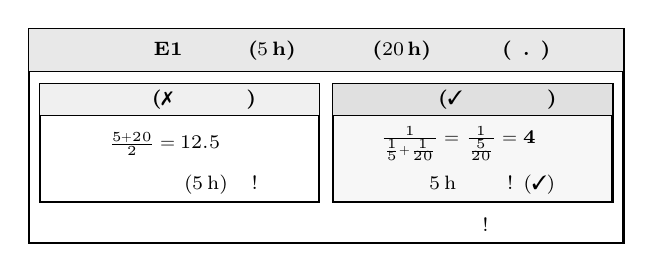
\begin{tikzpicture}[x=1cm, y=1cm, every node/.style={font=\scriptsize, text=black}]
  \draw[black, line width=0.9pt] (0,0) rectangle (7.55,2.72);
  \fill[gray!18] (0,2.18) rectangle (7.55,2.72);
  \draw[black, line width=0.6pt] (0,2.18) -- (7.55,2.18);
  \node at (3.775,2.45) {\textbf{បេសកកម្ម \en{E1}៖ បំពង់ទី១ ($5\unit{h}$) និងបំពង់ទី២ ($20\unit{h}$) បើករួមគ្នា (ទំ.៨៤)}};

  % Student A
  \draw[black, line width=0.7pt] (0.14,0.52) rectangle (3.68,2.02);
  \fill[gray!12] (0.14,1.62) rectangle (3.68,2.02);
  \draw[black, line width=0.45pt] (0.14,1.62) -- (3.68,1.62);
  \node at (1.91,1.82) {\textbf{សិស្ស ក (\ding{55} មធ្យមនព្វន្ធ)}};
  \node at (1.91,1.26) {$\tfrac{5 + 20}{2} = 12.5\text{ ម៉ោង}$};
  \node at (1.91,0.74) {យូរជាងបំពង់ទី១ ($5\unit{h}$) ទៀត!};

  % Student B
  \draw[black, line width=0.85pt, fill=gray!6] (3.86,0.52) rectangle (7.41,2.02);
  \fill[gray!24] (3.86,1.62) rectangle (7.41,2.02);
  \draw[black, line width=0.55pt] (3.86,1.62) -- (7.41,1.62);
  \node at (5.635,1.82) {\textbf{សិស្ស ខ (\ding{51} ប្រភាគលើប្រភាគ)}};
  \node at (5.635,1.26) {$\tfrac{1}{\frac{1}{5} + \frac{1}{20}} = \tfrac{1}{\frac{5}{20}} = \mathbf{4\text{ ម៉ោង}}$};
  \node at (5.635,0.74) {លឿនជាង $5\unit{h}$ សមហេតុផល! (\ding{51})};

  \node at (3.775,0.24) {\textbf{គន្លឹះ៖} អត្រារួមគិតតាមប្រភាគលើប្រភាគ មិនមែនបូកម៉ោងចែកពីរទេ!};
\end{tikzpicture}}

% ២. E2 Explore: លំហាត់គំរូ ១ (ទំ.៨៣–៨៤) សម្គាល់របារប្រភាគធំ និងសរសេរ x+1 ជា (x+1)/1
\newcommand{\figExploreRATSixSix}{%
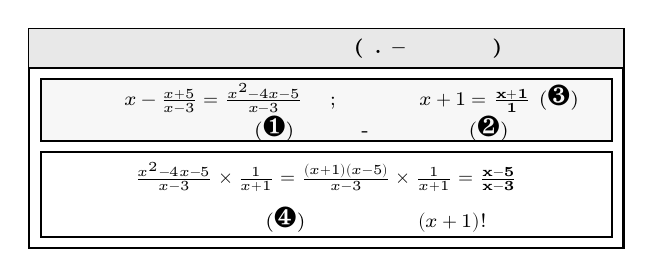
\begin{tikzpicture}[x=1cm, y=1cm, every node/.style={font=\scriptsize, text=black}]
  \draw[black, line width=0.9pt] (0,0) rectangle (7.55,2.78);
  \fill[gray!18] (0,2.28) rectangle (7.55,2.78);
  \draw[black, line width=0.6pt] (0,2.28) -- (7.55,2.28);
  \node at (3.775,2.53) {\textbf{បំប្លែងប្រភាគលើប្រភាគជាវិធីគុណចម្រាស (ទំ.៨៣–៨៤ លំហាត់គំរូ ១)}};

  \draw[black, line width=0.7pt, fill=gray!6] (0.15,1.36) rectangle (7.40,2.14);
  \node at (3.775,1.90) {ភាគយកធំ៖ $x - \tfrac{x+5}{x-3} = \tfrac{x^2 - 4x - 5}{x - 3}$ \quad ; \quad ភាគបែងធំ៖ $x + 1 = \mathbf{\tfrac{x + 1}{1}}$ (\cnum{3})};
  \node at (3.775,1.52) {សម្គាល់របារប្រភាគធំ (\cnum{1}) រួចបង្រួមលើ-ក្រោមជាប្រភាគមួយៗ (\cnum{2})};

  \draw[black, line width=0.75pt] (0.15,0.14) rectangle (7.40,1.22);
  \node at (3.775,0.90) {$\tfrac{x^2 - 4x - 5}{x - 3} \times \tfrac{1}{x + 1} = \tfrac{(x + 1)(x - 5)}{x - 3} \times \tfrac{1}{x + 1} = \mathbf{\tfrac{x - 5}{x - 3}}$};
  \node at (3.775,0.36) {គុណនឹងចម្រាសក្រោម (\cnum{4}) រួចដាក់កត្តាសម្រួល $(x + 1)$!};
\end{tikzpicture}}

% ៣. E3 Explain: វិធានប្រភាគលើប្រភាគ និងធនាគារហេតុផល ①–④ (ទំ.៨៣)
\newcommand{\figExplainRATSixSix}{%
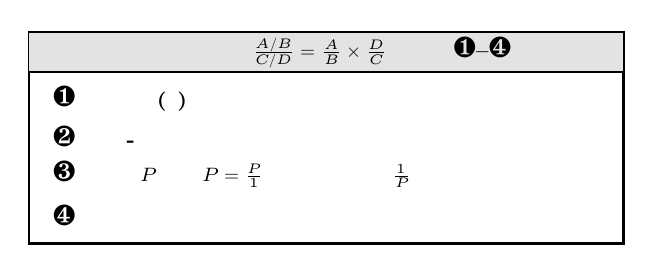
\begin{tikzpicture}[x=1cm, y=1cm, every node/.style={font=\scriptsize, text=black}]
  \draw[black, line width=0.95pt] (0,0) rectangle (7.55,2.68);
  \fill[gray!22] (0,2.18) rectangle (7.55,2.68);
  \draw[black, line width=0.65pt] (0,2.18) -- (7.55,2.18);
  \node at (3.775,2.43) {\textbf{វិធានប្រភាគលើប្រភាគ $\tfrac{A/B}{C/D} = \tfrac{A}{B}\times\tfrac{D}{C}$ និងហេតុផល \cnum{1}--\cnum{4}}};

  \node[anchor=west] at (0.18,1.84) {\cnum{1} \textbf{របារប្រភាគធំ (មេ)៖} បែងចែកច្បាស់រវាងភាគយកធំ និងភាគបែងធំ។};
  \node[anchor=west] at (0.18,1.36) {\cnum{2} \textbf{បង្រួមលើ-ក្រោមសិន៖} តម្រូវឱ្យលើនិងក្រោមក្លាយជាប្រភាគមួយៗ។};
  \node[anchor=west] at (0.18,0.88) {\cnum{3} \textbf{ករណីពហុធា $P$៖} សរសេរ $P = \tfrac{P}{1}$ ដើម្បីងាយត្រឡប់ចម្រាស $\tfrac{1}{P}$។};
  \node[anchor=west] at (0.18,0.36) {\cnum{4} \textbf{គុណចម្រាសក្រោម៖} ប្រភាគលើគុណចម្រាសក្រោម រួចសម្រួលកត្តា។};
\end{tikzpicture}}

% ៤. E4 Elaborate: រូបអាងទឹកបំពង់ ២ (ទំ.៨៤ លំហាត់គំរូ ២) និងប្រតិបត្តិ ខ (ទំ.៨៤)
\newcommand{\figElaborateRATSixSix}{%
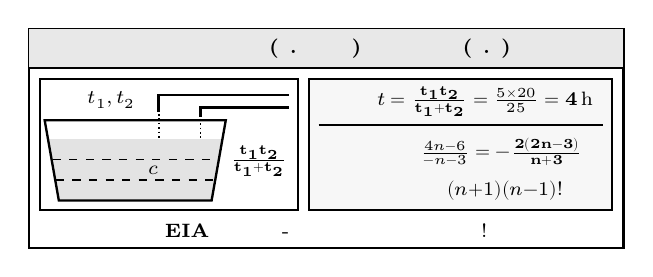
\begin{tikzpicture}[x=1cm, y=1cm, every node/.style={font=\scriptsize, text=black}]
  \draw[black, line width=0.9pt] (0,0) rectangle (7.55,2.78);
  \fill[gray!18] (0,2.28) rectangle (7.55,2.78);
  \draw[black, line width=0.6pt] (0,2.28) -- (7.55,2.28);
  \node at (3.775,2.53) {\textbf{រូបមន្តបំពង់ទឹកទាំងពីរ (ទំ.៨៤ គំរូ ២) និងប្រតិបត្តិ ខ (ទំ.៨៤)}};

  % Left: B&W Water Tank with Two Taps (matching Book p. 84)
  \draw[black, line width=0.75pt] (0.14,0.48) rectangle (3.42,2.14);
  % Tank trapezoid
  \fill[gray!22] (0.38,0.60) -- (2.32,0.60) -- (2.46,1.38) -- (0.24,1.38) -- cycle;
  \draw[black, line width=0.85pt] (0.20,1.62) -- (0.38,0.60) -- (2.32,0.60) -- (2.50,1.62) -- cycle;
  \draw[black, dashed, line width=0.45pt] (0.30,1.12) -- (2.40,1.12);
  \draw[black, dashed, line width=0.45pt] (0.34,0.86) -- (2.36,0.86);
  % Two Pipes & Taps
  \draw[black, line width=1.0pt] (3.30,1.94) -- (1.65,1.94) -- (1.65,1.72);
  \draw[black, line width=1.0pt] (3.30,1.78) -- (2.18,1.78) -- (2.18,1.66);
  \draw[black, densely dotted, line width=0.6pt] (1.65,1.70) -- (1.65,1.40);
  \draw[black, densely dotted, line width=0.6pt] (2.18,1.64) -- (2.18,1.40);
  \node at (1.05,1.88) {$t_1, t_2$};
  \node at (1.35,0.98) {\textbf{ចំណុះ $c$}};
  \node at (2.92,1.10) {$\mathbf{\tfrac{t_1 t_2}{t_1+t_2}}$};

  % Right: Formula + Practice B
  \draw[black, line width=0.8pt, fill=gray!6] (3.56,0.48) rectangle (7.41,2.14);
  \node at (5.485,1.86) {\textbf{គំរូ ២៖} $t = \mathbf{\tfrac{t_1 t_2}{t_1 + t_2}} = \tfrac{5\times 20}{25} = \mathbf{4\unit{h}}$};
  \draw[black, line width=0.45pt] (3.68,1.56) -- (7.29,1.56);
  \node at (5.485,1.22) {\textbf{ប្រតិបត្តិ ខ៖} $\tfrac{4n - 6}{-n - 3} = \mathbf{-\tfrac{2(2n - 3)}{n + 3}}$};
  \node at (5.485,0.72) {សម្រួលភាគបែងតូច $(n{+}1)(n{-}1)$!};

  \node at (3.775,0.22) {\textbf{\en{EIA}៖} ភាគបែងតូចលើ-ក្រោមដូចគ្នា ផលចែកស្មើផលធៀបភាគយកតូច!};
\end{tikzpicture}}

% ៥. E5 Evaluate: ជម្រើសវិនិច្ឆ័យ A-D សម្រាប់ (2/x) / (1 + 1/x)
\newcommand{\figExitRATSixSix}{%
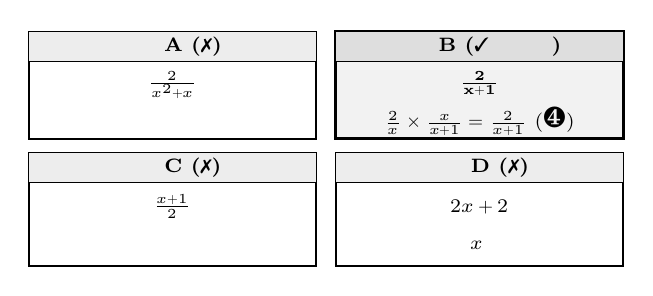
\begin{tikzpicture}[x=1cm, y=1cm, every node/.style={font=\scriptsize, text=black}]
  % Choice A
  \draw[black, line width=0.8pt] (0,1.62) rectangle (3.65,2.98);
  \fill[gray!14] (0,2.60) rectangle (3.65,2.98);
  \draw[black, line width=0.5pt] (0,2.60) -- (3.65,2.60);
  \node at (1.825,2.79) {\textbf{ជម្រើស \en{A} (\ding{55})}};
  \node at (1.825,2.30) {$\tfrac{2}{x^2 + x}$};
  \node at (1.825,1.84) {ភ្លេចត្រឡប់ចម្រាសប្រភាគក្រោម};

  % Choice B (Correct)
  \draw[black, line width=1.0pt, fill=gray!10] (3.90,1.62) rectangle (7.55,2.98);
  \fill[gray!26] (3.90,2.60) rectangle (7.55,2.98);
  \draw[black, line width=0.55pt] (3.90,2.60) -- (7.55,2.60);
  \node at (5.725,2.79) {\textbf{ជម្រើស \en{B} (\ding{51} ត្រឹមត្រូវ)}};
  \node at (5.725,2.32) {$\mathbf{\tfrac{2}{x + 1}}$};
  \node at (5.725,1.84) {$\tfrac{2}{x} \times \tfrac{x}{x + 1} = \tfrac{2}{x + 1}$ (\cnum{4})};

  % Choice C
  \draw[black, line width=0.8pt] (0,0) rectangle (3.65,1.44);
  \fill[gray!14] (0,1.06) rectangle (3.65,1.44);
  \draw[black, line width=0.5pt] (0,1.06) -- (3.65,1.06);
  \node at (1.825,1.25) {\textbf{ជម្រើស \en{C} (\ding{55})}};
  \node at (1.825,0.76) {$\tfrac{x + 1}{2}$};
  \node at (1.825,0.26) {ត្រឡប់ខុសប្រភាគលើជំនួសក្រោម};

  % Choice D
  \draw[black, line width=0.8pt] (3.90,0) rectangle (7.55,1.44);
  \fill[gray!14] (3.90,1.06) rectangle (7.55,1.44);
  \draw[black, line width=0.5pt] (3.90,1.06) -- (7.55,1.06);
  \node at (5.725,1.25) {\textbf{ជម្រើស \en{D} (\ding{55})}};
  \node at (5.725,0.76) {$2x + 2$};
  \node at (5.725,0.26) {ច្រឡំសម្រួល $x$ ហើយគុណបញ្ចូល};
\end{tikzpicture}}

% ============================================================================
% ៦. ចាប់ផ្ដើមឯកសារ (Document Body)
% ============================================================================
\begin{document}
\fontsize{10pt}{15.2pt}\selectfont

% --- ក្បាលរដ្ឋបាល ៣ ជួរ ---
{\muol
មន្ទីរអប់រំ យុវជន និងកីឡា ខេត្តកំពង់ធំ\\
ការិយាល័យអប់រំ យុវជន និងកីឡា ស្រុកកំពង់ស្វាយ\\
អនុវិទ្យាល័យព្រះក្រសាំង\par}

\vspace{-6pt}
\begin{center}
  \khmflourish\\[2pt]
  {\muol\fontsize{12pt}{18pt}\selectfont កិច្ចតែងការបង្រៀន}
\end{center}
\vspace{2pt}

% --- ព័ត៌មានទូទៅ ---
\begin{tabular}{@{}l@{\hspace{1.8cm}}l@{}}
  \ditem \textbf{មុខវិជ្ជា៖} គណិតវិទ្យា & \ditem \textbf{ថ្នាក់ទី៖} \enbf{8} (ម៉ោងទី៦ បញ្ចប់មេរៀនទី៦) \\
  \multicolumn{2}{@{}l@{}}{\ditem \textbf{ជំពូកទី២ (ពីជគណិត) -- មេរៀនទី៦៖} កន្សោមសនិទាន (សៀវភៅសិក្សាគោល ទំព័រ \en{75--88})} \\
  \multicolumn{2}{@{}l@{}}{\ditem \textbf{ខ្លឹមសារបង្រៀន៖} \textbf{៦. កន្សោមសនិទានដែលមានទម្រង់ប្រភាគលើប្រភាគ} (ទំព័រ \en{83--84, 87})} \\
  \ditem \textbf{រយៈពេល៖} \en{50} នាទី (\en{1} ម៉ោងសិក្សា) & \ditem \textbf{កាលបរិច្ឆេទ៖} ថ្ងៃសៅរ៍ ទី១៩ ខែធ្នូ ឆ្នាំ២០២៦
\end{tabular}

\vspace{5pt}

% --- I. វត្ថុបំណង ---
{\muol \enbf{I.} វត្ថុបំណង}\par
\vspace{2pt}
ក្រោយពីបញ្ចប់មេរៀននេះ សិស្សមានសមត្ថភាព៖
\begin{itemize}[leftmargin=1.35cm, label=\wcirc, itemsep=1pt, topsep=2pt, parsep=0pt]
  \item \textbf{វិជ្ជាសម្បទា៖} ប្រាប់និយមន័យ និងវិធានសម្រួលកន្សោមសនិទានដែលមានទម្រង់ប្រភាគលើប្រភាគ $\dfrac{\;\frac{A}{B}\;}{\frac{C}{D}} = \dfrac{A}{B} \times \dfrac{D}{C}$ ($B, C, D \neq 0$) បានត្រឹមត្រូវតាមសៀវភៅសិក្សាគោល (ទំព័រ ៨៣)។
  \item \textbf{បំណិនសម្បទា៖} សម្រួលកន្សោមសនិទានដែលមានទម្រង់ប្រភាគលើប្រភាគ និងដោះស្រាយចំណោទអត្រាការងាររួម (បំពង់ទឹកទាំងពីរ $\dfrac{t_1 t_2}{t_1 + t_2}$) ក្នុងសន្លឹកកិច្ចការបំពេញចន្លោះបានត្រឹមត្រូវ។
  \item \textbf{ចរិយាសម្បទា៖} មានទម្លាប់សម្គាល់របារប្រភាគធំ (មេ) ឱ្យច្បាស់លាស់ សរសេរពហុធាជាប្រភាគភាគបែង $1$ និងផ្ទៀងផ្ទាត់ភាពសមហេតុផលនៃចម្លើយចំណោទជីវភាពរស់នៅ។
\end{itemize}

\vspace{4pt}

% --- II. សម្ភារៈឧបទេស (Zero-LCD & Fill-In Worksheet Mode) ---
{\muol \enbf{II.} សម្ភារៈឧបទេស}\par
\vspace{2pt}
\begin{itemize}[leftmargin=1.35cm, label=\wcirc, itemsep=1pt, topsep=2pt, parsep=0pt]
  \item \textbf{សម្រាប់គ្រូ៖} សៀវភៅសិក្សាគោលគណិតវិទ្យាថ្នាក់ទី៨ (ទំព័រ ៨៣–៨៤, ៨៧) ក្ដារខៀន ដីសស និងប្លង់ក្ដារខៀន ៣ ផ្នែក (គ្មានស្លាយ \en{LCD} និងគ្មានឧបករណ៍កាត់បិទ)។
  \item \textbf{សម្រាប់សិស្ស៖} \textbf{សន្លឹកកិច្ចការសិស្សបំពេញចន្លោះ ស-ខ្មៅ} (បោះពុម្ពសងខាង ១ សន្លឹកក្នុងម្នាក់ សម្រាប់បំពេញតាមជំហាន \en{E1--E5}) សៀវភៅសិក្សាគោល និងប៊ិច។
\end{itemize}

\vspace{4pt}

% --- III. វិធីសាស្រ្តបង្រៀន ---
{\muol \enbf{III.} វិធីសាស្រ្តបង្រៀន}\par
\vspace{2pt}
\begin{itemize}[leftmargin=1.35cm, label=\wcirc, itemsep=1pt, topsep=2pt, parsep=0pt]
  \item គោលវិធីសិស្សមជ្ឈមណ្ឌល តាមលំនាំរិះរក \textbf{\en{5Es} (\en{Engage, Explore, Explain, Elaborate, Evaluate})} ដោយប្រើសន្លឹកកិច្ចការបំពេញចន្លោះជាគោល។
  \item យុទ្ធសាស្ត្រផ្អែកលើការស្រាវជ្រាវគរុកោសល្យអន្តរជាតិ៖ \textbf{ការសម្គាល់របារប្រភាគធំ និងការបំប្លែងជាផលគុណចម្រាស} (\en{Tirosh, 2000}) និង \textbf{ការប្រៀបធៀបឧទាហរណ៍ខុស-ត្រូវក្នុងចំណោទអត្រារួម} (\en{Booth et al., 2013; Rittle-Johnson \& Star, 2007})។
\end{itemize}

\vspace{4pt}

% --- IV. ដំណើរការបង្រៀន (50 នាទី) ---
{\muol \enbf{IV.} ដំណើរការបង្រៀន}\par
\vspace{2pt}

\renewcommand{\arraystretch}{1.15}
\begin{longtable}{|L{5.50cm}|L{7.90cm}|L{4.80cm}|}
\hline
\multicolumn{1}{|c|}{\cellcolor{headgray}\textbf{សកម្មភាពគ្រូ}} &
\multicolumn{1}{c|}{\cellcolor{headgray}\textbf{ខ្លឹមសារមេរៀន}} &
\multicolumn{1}{c|}{\cellcolor{headgray}\textbf{សកម្មភាពសិស្ស}} \\
\hline
\endfirsthead

\hline
\multicolumn{1}{|c|}{\cellcolor{headgray}\textbf{សកម្មភាពគ្រូ}} &
\multicolumn{1}{c|}{\cellcolor{headgray}\textbf{ខ្លឹមសារមេរៀន}} &
\multicolumn{1}{c|}{\cellcolor{headgray}\textbf{សកម្មភាពសិស្ស}} \\
\hline
\endhead

\hline
\endfoot

% ==================== ជំហានទី១ (2min) ====================
\stepheader{ជំហានទី១ \enbf{(}រដ្ឋបាលថ្នាក់\enbf{)} \timenote{(2min)}}
$\bullet$ ពិនិត្យអនាម័យ សណ្ដាប់ធ្នាប់ និងវត្តមានសិស្ស \par
$\bullet$ ចែក \textbf{សន្លឹកកិច្ចការបំពេញចន្លោះ} ដល់សិស្សគ្រប់គ្នា
&
$\bullet$ វត្តមានសិស្ស៖ \dotfill នាក់ (អវត្តមាន៖ \dotfill នាក់) \par
$\bullet$ ត្រៀមសៀវភៅគោល (ទំ.៨៣–៨៤) និងសន្លឹកកិច្ចការសិស្ស
&
$\circ$ ប្រធានថ្នាក់រាយការណ៍វត្តមាន \par
$\circ$ ទទួលសន្លឹកកិច្ចការ និងសរសេរឈ្មោះ \\
\hline

% ==================== ជំហានទី២ (9min) ====================
\stepheader{ជំហានទី២ \enbf{(}ពិនិត្យកិច្ចការចាស់ \enbf{+} រំលឹកមេរៀន \enbf{+} \enbf{E1}\enbf{)} \timenote{(9min)}}
\redsub{$\bullet$ ពិនិត្យកិច្ចការផ្ទះ} \timenote{(កុំឱ្យលើស 3min)} \par
$\bullet$ ហៅសិស្ស ២ នាក់ឡើងសរសេរចម្លើយកិច្ចការផ្ទះម៉ោងមុន (ទំ.៨៦ \en{\#8} ខ, ឆ, ឈ និង ទំ.៨៨ \en{\#14} ក, គ) លើក្ដារខៀនឆ្វេង
&
\textbf{កំណែកិច្ចការផ្ទះ (ទំ.៨៦ \en{\#8} និង ទំ.៨៨ \en{\#14})៖} \par
$\bullet$ \en{\#8} ខ) $\dfrac{3x + 7y}{6}$ \quad ; \quad ឆ) $\dfrac{b}{b-4} - \dfrac{b}{b-4} = 0$ \quad ; \quad ឈ) $\dfrac{5a + 4}{6(a - 4)}$ \par
$\bullet$ \en{\#14} ក) $\dfrac{1}{8} - \dfrac{1}{9} = \dfrac{1}{8\times 9}$ \quad ; \quad គ) $\dfrac{1}{18} - \dfrac{1}{19} = \dfrac{1}{18\times 19} \Rightarrow a = 18, b = 19$
&
$\circ$ សិស្ស ២ នាក់ឡើងសរសេរចម្លើយ \par
$\circ$ ផ្ទៀងផ្ទាត់ និងកែចម្លើយក្នុងសៀវភៅ \\[3pt]

\redsub{$\bullet$ រំលឹកមេរៀនចាស់} \timenote{(3min)} \par
$\bullet$ សួរផ្ទាល់មាត់រំលឹកវិធីចែកប្រភាគ និងការបូកប្រភាគភាគបែងខុសគ្នា \par
\hspace*{0.3em}– សំណួរ៖ «តើ $\dfrac{2}{3} \div \dfrac{1}{3}$ ស្មើប៉ុន្មាន? ហើយ $\dfrac{1}{5} + \dfrac{1}{20}$ ស្មើប៉ុន្មាន?»
&
\textbf{រំលឹកវិធីចែកប្រភាគ និងផលបូកអត្រា៖} \par
$\bullet$ ចែកប្រភាគ៖ $\dfrac{2}{3} \div \dfrac{1}{3} = \dfrac{2}{3} \times \dfrac{3}{1} = 2$ (គុណនឹងចម្រាសនៃតួចែក)។ \par
$\bullet$ បូកប្រភាគ៖ $\dfrac{1}{5} + \dfrac{1}{20} = \dfrac{4 + 1}{20} = \dfrac{5}{20} = \dfrac{1}{4}$ ។
&
$\circ$ ឆ្លើយផ្ទាល់មាត់៖ $\dfrac{2}{3} \div \dfrac{1}{3} = 2$ និង $\dfrac{1}{5} + \dfrac{1}{20} = \dfrac{1}{4}$ \\[3pt]

\fiveE{E1 - Engage} \timenote{(3min)} \par
$\bullet$ លើកបញ្ហាបំពង់ទឹកទាំងពីរ (លំហាត់គំរូ ២ ទំ.៨៤៖ $t_1 = 5\unit{h}, t_2 = 20\unit{h}$) ឱ្យសិស្សវិនិច្ឆ័យចម្លើយ \textbf{សិស្ស ក} និង \textbf{សិស្ស ខ}
&
\textbf{៦. កន្សោមសនិទានដែលមានទម្រង់ប្រភាគលើប្រភាគ (ទំ.៨៣)} \par
$\bullet$ \textbf{បេសកកម្ម \en{E1}៖} បំពង់ទី១ បង្ហូរពេញអាងក្នុង $5\unit{h}$ ឯបំពង់ទី២ ក្នុង $20\unit{h}$ ។ បើបើករួមគ្នា តើប្រើពេលប៉ុន្មានម៉ោង? (\textbf{សិស្ស ក៖} $12.5\unit{h}$ ទល់នឹង \textbf{សិស្ស ខ៖} $4\unit{h}$)
&
$\circ$ គូសធីកជ្រើសរើសចម្លើយ និងពិភាក្សាភាពសមហេតុផលក្នុងប្រអប់ \en{E1} \\[3pt]

$\bullet$ សួរឆ្កឹះ៖ «បើបំពង់ទី១ តែឯងប្រើពេលតែ $5\unit{h}$ តើបើកពីរបំពង់ជួយគ្នាអាចយូរដល់ $12.5\unit{h}$ ដែរឬទេ?»
&
\cfig{\figEngageRATSixSix}
&
$\circ$ ភ្ញាក់ខ្លួនថាមិនអាចយូរជាង $5\unit{h}$ ឡើយ! ចូលរៀនទម្រង់ប្រភាគលើប្រភាគ \\
\hline

% ==================== ជំហានទី៣ (17min) ====================
\stepheader{ជំហានទី៣ \enbf{(}មេរៀនថ្មី៖ \enbf{E2 + E3}\enbf{)} \timenote{(17min)}}
\fiveE{E2 - Explore} \timenote{(11min)} \par
$\bullet$ \textbf{ផ្នែក \en{E2-A} (៥ នាទី)៖} ឱ្យសិស្សធ្វើការជាដៃគូបំពេញចន្លោះប្រតិបត្តិ ក (ទំ.៨៤) និងឧទាហរណ៍ទំ.៨៣ លើសន្លឹកកិច្ចការទំព័រ ១
&
\textbf{សកម្មភាពរុករកទី១ (\en{E2-A})៖ ពីប្រភាគលេខទៅកន្សោមសនិទាន (ទំ.៨៣–៨៤)} \par
$\bullet$ \textbf{១) ប្រតិបត្តិ ក (ទំ.៨៤)៖} $\dfrac{1 - \frac{1}{3}}{\frac{1}{2} - \frac{1}{6}} = \dfrac{\;\frac{2}{3}\;}{\frac{1}{3}} = \dfrac{2}{3} \times \dfrac{3}{1} = \mathbf{2}$ ។ \par
$\bullet$ \textbf{២) ឧទាហរណ៍ (ទំ.៨៣)៖} $\dfrac{\frac{1}{a} + \frac{1}{b}}{\frac{b}{2a} - \frac{a}{2b}} = \dfrac{\frac{a + b}{ab}}{\frac{b^2 - a^2}{2ab}} = \dfrac{a + b}{ab} \times \dfrac{2ab}{(b + a)(b - a)} = \mathbf{\dfrac{2}{b - a}}$ ។
&
$\circ$ បង្រួមភាគយកធំ និងភាគបែងធំជាប្រភាគមួយៗ រួចគុណនឹងចម្រាសប្រភាគក្រោម \\[3pt]

$\bullet$ \textbf{ផ្នែក \en{E2-B} (៦ នាទី)៖} ណែនាំលំហាត់គំរូទី ១ (ទំ.៨៣–៨៤) ដែលភាគបែងធំជាពហុធា $x + 1$ \par
\hspace*{0.3em}– សំណួរ៖ «តើគួរសរសេរ $x + 1$ ជាប្រភាគដូចម្ដេចដើម្បីងាយត្រឡប់ចម្រាស?»
&
\textbf{សកម្មភាពរុករកទី២ (\en{E2-B})៖ ភាគបែងធំជាពហុធា (លំហាត់គំរូ ១ ទំ.៨៣–៨៤)} \par
$\bullet$ សម្រួល $\dfrac{x - \frac{x + 5}{x - 3}}{x + 1}$៖ \par
\hspace*{0.4em}– បង្រួមភាគយកធំ៖ $x - \dfrac{x + 5}{x - 3} = \dfrac{x(x - 3) - (x + 5)}{x - 3} = \dfrac{x^2 - 4x - 5}{x - 3}$ \par
\hspace*{0.4em}– សរសេរភាគបែងធំជា $\dfrac{x + 1}{1}$ រួចគុណនឹងចម្រាស $\dfrac{1}{x + 1}$ ។
&
$\circ$ សរសេរ $x + 1 = \dfrac{x + 1}{1}$ ពន្លាតភាគយកដោយដាក់វង់ក្រចក $-(x + 5)$ រួចដាក់ជាកត្តា \\[3pt]

$\bullet$ គូសតារាងសង្ខេបលើក្ដារខៀន ឱ្យសិស្សផ្ទៀងផ្ទាត់ការដាក់កត្តា $(x + 1)(x - 5)$ និងសម្រួល
&
\cfig{\figExploreRATSixSix}
&
$\circ$ សម្រួលកត្តារួម $(x + 1)$ បានចម្លើយ $\dfrac{x - 5}{x - 3}$ \\[3pt]

\fiveE{E3 - Explain} \timenote{(6min)} \par
$\bullet$ ឱ្យតំណាងដៃគូ ២ ក្រុមឡើងបកស្រាយ \en{E2-A} និង \en{E2-B} រួចទាញវិធានសម្រួលប្រភាគលើប្រភាគ (ទំ.៨៣)
&
\textbf{វិធានសម្រួលកន្សោមប្រភាគលើប្រភាគ (ទំ.៨៣)៖} \par
$\bullet$ កន្សោមដែលមានភាគយក ឬភាគបែងជាប្រភាគ ហៅថា \textbf{ប្រភាគលើប្រភាគ}។ \par
$\bullet$ បង្រួមភាគយកធំជាប្រភាគមួយ $\dfrac{A}{B}$ និងភាគបែងធំជាប្រភាគមួយ $\dfrac{C}{D}$ រួចគណនា៖ $\dfrac{\;\frac{A}{B}\;}{\frac{C}{D}} = \dfrac{A}{B} \times \dfrac{D}{C} = \mathbf{\dfrac{A \cdot D}{B \cdot C}}$ ($B, C, D \neq 0$)។
&
$\circ$ តំណាងក្រុមឡើងបកស្រាយ \par
$\circ$ បំពេញប្រអប់វិធាន \en{E3} លើសន្លឹកកិច្ចការទំព័រ ១ \\[3pt]

$\bullet$ សង្ខេប \textbf{ធនាគារហេតុផល \cnum{1}--\cnum{4}} លើក្ដារខៀនកណ្ដាលទុកជាគោលការណ៍យោង
&
\cfig{\figExplainRATSixSix}
&
$\circ$ កត់ចំណាំហេតុផល \cnum{1}--\cnum{4} ទុកការពារកំហុសត្រឡប់ប្រភាគខុស \\
\hline

% ==================== ជំហានទី៤ (20min) ====================
\stepheader{ជំហានទី៤ \enbf{(}ពង្រឹងពុទ្ធិ និងវាយតម្លៃ៖ \enbf{E4 + E5}\enbf{)} \timenote{(20min)}}
\fiveE{E4 - Elaborate} \timenote{(10min)} \par
$\bullet$ ណែនាំលំហាត់គំរូទី ២ (បំពង់ទឹកទាំងពីរ ទំ.៨៤) និងប្រតិបត្តិ ខ (ទំ.៨៤) លើសន្លឹកកិច្ចការទំព័រ ២ \par
$\bullet$ ឱ្យសិស្សស្រាយបញ្ជាក់រូបមន្តទូទៅ $\dfrac{t_1 t_2}{t_1 + t_2}$ រួចជំនួសលេខ $t_1 = 5, t_2 = 20$
&
\textbf{ការពង្រីកចំណេះដឹង (\en{E4})៖ លំហាត់គំរូ ២ និងប្រតិបត្តិ ខ (ទំ.៨៤)} \par
$\bullet$ \textbf{១) លំហាត់គំរូ ២ (បំពង់ទឹក ទំ.៨៤)៖} តាង $c$ ជាចំណុះអាង។ ក្នុង $1\unit{h}$ បំពង់ទាំងពីរបង្ហូរបាន $\dfrac{c}{t_1} + \dfrac{c}{t_2} = c\left(\dfrac{1}{t_1} + \dfrac{1}{t_2}\right)$ ។ \par
\hspace*{0.4em}– រយៈពេលរួម៖ $t = \dfrac{c}{c\left(\frac{1}{t_1} + \frac{1}{t_2}\right)} = \dfrac{1}{\frac{t_2 + t_1}{t_1 t_2}} = \mathbf{\dfrac{t_1 t_2}{t_1 + t_2}}$ (ចំពោះ $5\unit{h}, 20\unit{h} \Rightarrow \mathbf{4\unit{h}}$)។
&
$\circ$ សម្រួលចំណុះ $c$ ចោល រួចគណនាប្រភាគលើប្រភាគឃើញរូបមន្ត $\dfrac{t_1 t_2}{t_1 + t_2}$ និង $t = 4\unit{h}$ \\[3pt]

$\bullet$ ឱ្យសិស្សគណនាប្រតិបត្តិ ខ (ទំ.៨៤) ដោយតម្រូវភាគបែងតូច $(n + 1)(n - 1)$ ទាំងលើទាំងក្រោម
&
$\bullet$ \textbf{២) ប្រតិបត្តិ ខ (ទំ.៨៤)៖} $\dfrac{\frac{5}{n + 1} - \frac{1}{n - 1}}{\frac{1}{n + 1} - \frac{2}{n - 1}} = \dfrac{\frac{5(n - 1) - (n + 1)}{(n + 1)(n - 1)}}{\frac{(n - 1) - 2(n + 1)}{(n + 1)(n - 1)}} = \dfrac{4n - 6}{-n - 3} = \mathbf{-\dfrac{2(2n - 3)}{n + 3}}$ ។
&
$\circ$ ពន្លាតភាគយកលើ-ក្រោម រួចសម្រួលភាគបែងតូច $(n+1)(n-1)$ ដែលដូចគ្នា \\[3pt]

$\bullet$ សួរសំណួរ \textbf{\en{EIA Looking-Back}}៖ «ហេតុអ្វីកត្តាភាគបែងតូច $(n+1)(n-1)$ ទាំងលើទាំងក្រោមអាចសម្រួលគ្នាអស់ភ្លាម?»
&
\cfig{\figElaborateRATSixSix}
&
$\circ$ ឆ្លើយសំណួរ \en{EIA}៖ ព្រោះពេលគុណនឹងចម្រាស $(n+1)(n-1)$ ឡើងលើ សម្រួលគ្នាបាន $1$! \\[3pt]

\fiveE{E5 - Evaluate} \timenote{(10min)} \par
$\bullet$ \textbf{ហ្វឹកហាត់ក្រុមតូច (៥ នាទី)៖} ឱ្យសិស្សធ្វើលំហាត់ទំ.៨៧ \en{\#9} (ក, គ, ឃ, ង) ក្នុងសន្លឹកកិច្ចការ \par
\hspace*{0.3em}– \textbf{ផ្អាកសួរ (\en{Pause-Review})៖} ផ្ទៀងផ្ទាត់ការដាក់កត្តា $5x^2 - 45 = 5(x-3)(x+3)$ ក្នុង \en{\#9} ង
&
\textbf{ហ្វឹកហាត់លំហាត់សៀវភៅគោល (ទំ.៨៧ លេខ ៩ ក, គ, ឃ, ង)៖} \par
$\bullet$ \en{\#9} ក) $\dfrac{\frac{1}{6} + \frac{1}{3}}{\frac{1}{5} + \frac{1}{5}} = \dfrac{\;\frac{1}{2}\;}{\frac{2}{5}} = \mathbf{\dfrac{5}{4}}$ \quad ; \quad គ) $\dfrac{\frac{5}{6} - \frac{5}{7}}{\frac{5}{6} + \frac{5}{7}} = \dfrac{\;\frac{5}{42}\;}{\frac{65}{42}} = \mathbf{\dfrac{1}{13}}$ \par
$\bullet$ \en{\#9} ឃ) $\dfrac{\;\frac{3}{x}\;}{\frac{1}{x} - \frac{1}{3x}} = \dfrac{\;\frac{3}{x}\;}{\frac{2}{3x}} = \mathbf{\dfrac{9}{2}}$ \quad ; \quad ង) $\dfrac{\frac{2x}{3} + 2}{\frac{5x}{3} - \frac{15}{x}} = \dfrac{\frac{2(x+3)}{3}}{\frac{5(x-3)(x+3)}{3x}} = \mathbf{\dfrac{2x}{5(x - 3)}}$
&
$\circ$ គណនាបំពេញចន្លោះជាក្រុម ៤ នាក់ និងផ្ទៀងផ្ទាត់ហេតុផល \cnum{1}--\cnum{4} ជាមួយមិត្តរួមតុ \\[3pt]

$\bullet$ \textbf{បិទបញ្ចប់បេសកកម្ម \en{E1} + ល្បឿនវិនិច្ឆ័យ \en{A--D} (៣ នាទី)៖} សួររកចម្លើយសម្រួលនៃ $\dfrac{\;\frac{2}{x}\;}{1 + \frac{1}{x}}$
&
\textbf{សំណួរវិនិច្ឆ័យរហ័ស (\en{60} វិនាទី)៖} តើកន្សោមប្រភាគលើប្រភាគ $\dfrac{\;\frac{2}{x}\;}{1 + \frac{1}{x}}$ សម្រួលទៅស្មើជម្រើសណា? (\textbf{ចម្លើយត្រូវ៖ \en{B}})
&
$\circ$ បញ្ជាក់ថាសិស្ស ខ ក្នុង \en{E1} ត្រឹមត្រូវ ($4\unit{h}$) \par
$\circ$ គូសរង្វង់ជម្រើស \en{B} និងប្រាប់មូលហេតុ \\[3pt]

$\bullet$ បង្ហាញការវិភាគជម្រើសទាំង ៤ លើក្ដារខៀន រួចឱ្យសិស្សធ្វើ \textbf{ប័ណ្ណចាកចេញបុគ្គល} (\en{2} នាទីចុងក្រោយ)
&
\cfig{\figExitRATSixSix}
&
$\circ$ ផ្ទៀងផ្ទាត់កំហុសត្រឡប់ខុសក្នុងជម្រើស \en{A, C, D} \\[3pt]

$\bullet$ ឱ្យសិស្សម្នាក់ៗធ្វើប្រអប់ \textbf{ប័ណ្ណចាកចេញ} (ទំ.៨៧ \en{\#9} ច) ដោយខ្លួនឯងមុនប្រមូលសន្លឹកកិច្ចការ
&
\textbf{ប័ណ្ណចាកចេញបុគ្គល (ទំ.៨៧ \en{\#9} ច)៖} \par
$\bullet$ សម្រួល៖ $\dfrac{k + \frac{k - 3}{k + 1}}{k - \frac{2}{k + 1}} = \dfrac{\frac{k^2 + 2k - 3}{k + 1}}{\frac{k^2 + k - 2}{k + 1}} = \dfrac{(k + 3)(k - 1)}{(k + 2)(k - 1)} = \mathbf{\dfrac{k + 3}{k + 2}}$ ។
&
$\circ$ គណនាប័ណ្ណចាកចេញបុគ្គលលើសន្លឹកកិច្ចការទំព័រ ២ រួចប្រគល់ជូនគ្រូ \\
\hline

% ==================== ជំហានទី៥ (≤2min) ====================
\stepheader{ជំហានទី៥ \enbf{(}កិច្ចការផ្ទះ \enbf{+} បណ្ដាំផ្ញើ\enbf{)}}
\timenote{ចំណាយពេលឱ្យតិចបំផុតកុំឱ្យលើស 2min} \par
$\bullet$ ណែនាំប្រអប់កិច្ចការផ្ទះបញ្ចប់មេរៀនទី៦ លើសន្លឹកកិច្ចការទំព័រ ២ (ទំ.៨៧ \en{\#9} និង \en{\#13})
&
\centering\textbf{កិច្ចការផ្ទះបញ្ចប់មេរៀនទី៦ (សៀវភៅគោល ទំ.៨៧ លេខ ៩ និង លេខ ១៣)}\par\raggedright
$\bullet$ \textbf{១) ទំ.៨៧ \en{\#9} ខ, ដ, ថ៖} សម្រួល $\dfrac{6 - \frac{5}{2} + \frac{3}{8}}{3 - \frac{5}{2} - \frac{7}{4}}$ , $\dfrac{a - \frac{a-b}{1+ab}}{1 + \frac{a(a-b)}{1+ab}}$ និង $\dfrac{1-2b}{1+\frac{1}{2b}} \div \dfrac{1+2b}{1-\frac{1}{2b}}$ ។ \par
$\bullet$ \textbf{២) ទំ.៨៧ \en{\#13} ក, ខ៖} រករយៈពេលកម្មករ ៣ នាក់ធ្វើការរួមគ្នា ($d_1 = 20, d_2 = 15, d_3 = 12$ ថ្ងៃ)។
&
$\circ$ គូសចំណាំកិច្ចការផ្ទះលើសន្លឹកកិច្ចការ \\[3pt]

$\bullet$ ផ្តាំផ្ញើឱ្យរំលឹកមេរៀនទី៦ ទាំងមូល (ទំ.៧៥–៨៨) និងអានមុនមេរៀនបន្ទាប់ក្នុងសៀវភៅគោល
&
$\bullet$ \textbf{បណ្ដាំផ្ញើ៖} ធ្វើកិច្ចការផ្ទះឱ្យបានគ្រប់គ្នា និងរំលឹកសង្ខេបរូបមន្តមេរៀនទី៦ កន្សោមសនិទានទាំងមូល ។
&
$\circ$ កត់ត្រាបណ្ដាំផ្ញើ ទុកសន្លឹកកិច្ចការក្នុងសៀវភៅ និងជម្រាបលាគ្រូ \\
\hline
\end{longtable}

\vspace{6pt}

% --- ហត្ថលេខា (Signature Block) ---
\begin{flushright}
  \begin{minipage}{9.5cm}
    \centering
    ថ្ងៃសៅរ៍ ១០កើត ខែមិគសិរ ឆ្នាំមមី អដ្ឋស័ក ពុទ្ធសករាជ ២៥៧០\\
    កំពង់ស្វាយ, ថ្ងៃទី១៩ ខែធ្នូ ឆ្នាំ២០២៦\\[4pt]
    {\muol គ្រូបង្រៀន}\\[32pt]
    \hfill{\muol ហុក ប៊ុនថែន}\hspace*{1.4cm}
  \end{minipage}
\end{flushright}

\end{document}
